\documentclass[
	% -- opções da classe memoir --
	12pt,				% tamanho da fonte
	openright,			% capítulos começam em pág ímpar (insere página vazia caso preciso)
	oneside,			% para impressão em frente e verso. Oposto a oneside
	a4paper,			% tamanho do papel.
	% -- opções da classe abntex2 --
	chapter=TITLE,		% títulos de capítulos convertidos em letras maiúsculas
	%section=TITLE,		% títulos de seções convertidos em letras maiúsculas
	%subsection=TITLE,	% títulos de subseções convertidos em letras maiúsculas
	%subsubsection=TITLE,% títulos de subsubseções convertidos em letras maiúsculas
	% -- opções do pacote babel --
	english,			% idioma adicional para hifenização
	french,				% idioma adicional para hifenização
	spanish,			% idioma adicional para hifenização
	brazil				% o último idioma é o principal do documento
	]{abntex2}
% ---
% Pacotes básicos 
% ---
\usepackage{lmodern}			% Usa a fonte Latin Modern
\usepackage{mathptmx}			% Usa a fonte Times New Roman
\usepackage[T1]{fontenc}		% Selecao de codigos de fonte.
\usepackage[utf8]{inputenc}		% Codificacao do documento (conversão automática dos acentos)
\usepackage{lastpage}			% Usado pela Ficha catalográfica
\usepackage{indentfirst}		% Indenta o primeiro parágrafo de cada seção.
\usepackage{color}				% Controle das cores
\usepackage{graphicx}			% Inclusão de gráficos
\usepackage{subcaption}				% Inclusão de gráficos lado a lado
\usepackage{microtype} 			% para melhorias de justificação
\usepackage{tabularx,ragged2e}	% Para inserir tabelas
\usepackage{multirow}			% Para mesclar células
\usepackage[dvipsnames,table,xcdraw]{xcolor}		% Permite adicionar cores nas linhas de tabelas
\usepackage{fancyvrb}			% Permite adicionar arquivos de texto
\usepackage[portuguese, ruled, linesnumbered]{algorithm2e} % Uso de algoritmos
\usepackage{amsfonts}			% Permite usar notação de conjuntos
\usepackage{amsmath}			% Permite citar equações
\usepackage{amsthm}				% Permite criar teoremas e experimentos
\usepackage[font={bf, small}, labelsep=endash, labelfont=bf]{caption}	% Faz legenda de figuras ficarem em negrito
\usepackage{cancel}				% Permite fazer expressão tendendo a zero
\usepackage{epstopdf}			% Converte eps para pdf
\usepackage[final]{pdfpages}
\usepackage{hyperref}
\usepackage{fancybox}
\usepackage{float}



\newcolumntype{L}{>{\RaggedRight\arraybackslash}X}
% ---
% ---
% Pacotes adicionais, usados apenas no âmbito do Modelo Canônico do abnteX2
% ---
\usepackage{lipsum}				% para geração de dummy text
% ---
% ---
% Pacotes de citações
% ---
%\usepackage[brazilian,hyperpageref]{backref}	 % Paginas com as citações na bibl
\usepackage[alf, abnt-emphasize=bf]{abntex2cite}	% Citações padrão ABNT
% ---
% Customizações para o layout da UFPA
% ---
\usepackage{modelo-ufpa/ufpa}
% Muda o título de lista de ilustrações para lista de figuras
\addto\captionsbrazil{%
  \renewcommand{\listfigurename}%
    {Lista de Ilustrações}%
	\renewcommand{\listtablename}%
    {Lista de Tabelas}%
}
% Permite utilizar figuras sem precisar colocar o caminho absoluto
\graphicspath{{imagens/}}
% Define o ambiente de experimentos
\theoremstyle{definition}
\newtheorem{experimento}{Experimento}[section]
\newcommand{\experimentoautorefname}{Experimento}


% --------------------------------------------------------------
% Informações do TRABALHO
% --------------------------------------------------------------
\universidade{UNIVERSIDADE FEDERAL DO PARÁ}
\instituto{INSTITUTO DE TECNOLOGIA}
\faculdade{FACULDADE DE COMPUTAÇÃO E TELECOMUNICAÇÕES}
%\curso{CURSO DE BACHARELADO EM SISTEMAS DE INFORMAÇÃO}
\titulo{RELATÓRIO DE SISTEMAS OPERACIONAIS}
\autor{
%\begin{tabular}{l l}
    DAVID PINHEIRO DE SOUSA - 202207040045 \\
    JOAO VICTOR SANTOS BRITO FERREIRA - 202207040028 \\
    JOEL TAVARES MIRANDA - 202206840054 \\
    KAUAN MIRANDA TAVARES - 202206840033 \\
    MARCO ANTONIO DO ESPIRITO SANTO MAUES JUNIOR - 202206840038 \\
%\end{tabular}
}
\local{Belém}
\data{2023}
\orientador{Prof. Dr. Diego Lisboa Cardoso}
\tipotrabalho{Monografia}

% o nome da instituição e a área de concentração 
\preambulo{Relatório do trabalho 3 de Sistemas Operacionais.}
%\sobrenome{Sobrenome}
%\nome{Nome}
%\palavraschave
%\datadadefesa{Data da Defesa: 09 de Março de 2017}%07 de Dezembro de 2016}
\conceito{Conceito: Excelente}
\faculdadedoorientador{Faculdade de Biotecnologia - UFPA}
\primeiromembrodabanca{Prof. Dr. Nome Sobrenome}
\faculdadedoprimeiromembrodabanca{Faculdade de Computação - UFPA}
\segundomembrodabanca{Prof. Dra. Nome Sobrenome}
\faculdadedosegundomembrodabanca{Faculdade de Biotecnologia - UFPA}
% -------------------------------------------------------------------------
% ---
% Configurações de aparência do PDF final
% alterando o aspecto da cor azul
\definecolor{blue}{RGB}{41,5,195}
% informações do PDF
\makeatletter
\hypersetup{
     	%pagebackref=true,
		pdftitle={\imprimirtitulo}, 
		pdfauthor={\imprimirautor},
    	pdfsubject={\imprimirpreambulo},
	    pdfcreator={LaTeX with abnTeX2},
		pdfkeywords={\imprimirpalavraschave}, 
		colorlinks=true,       		% false: boxed links; true: colored links
    	linkcolor=black,          	% color of internal links
    	citecolor=black,        		% color of links to bibliography
    	filecolor=magenta,      		% color of file links
		urlcolor=blue,
		bookmarksdepth=4,
        breaklinks=true
}
\makeatother
% --- 
% Espaçamentos entre linhas e parágrafos 
% --- 
% O tamanho do parágrafo é dado por:
\setlength{\parindent}{1.3cm}
% Controle do espaçamento entre um parágrafo e outro:
\setlength{\parskip}{0.2cm}  % tente também \onelineskip
% compila o indice
% ---
\makeindex
% ---

% -------------------------------------------------------------------------
% ---------------------------INICIO DO DOCUMENTO---------------------------
% -------------------------------------------------------------------------
\begin{document}
% Seleciona o idioma do documento (conforme pacotes do babel)
\selectlanguage{brazil}
% Retira espaço extra obsoleto entre as frases.
\frenchspacing 
% ----------------------------------------------------------
% ELEMENTOS PRÉ-TEXTUAIS
% ----------------------------------------------------------
% \pretextual

% ---
% Capa
% ---
\imprimircapa
% ---

% ---
% Folha de rosto

\imprimirfolhaderosto

\newpage

\setlength{\absparsep}{18pt} % ajusta o espaçamento dos parágrafos do resumo

\pdfbookmark[0]{\contentsname}{toc}
\tableofcontents*
\cleardoublepage
% ---
% ---------------------------------------------------------
% ELEMENTOS TEXTUAIS
% ----------------------------------------------------------
\textual

% ----------------------------------------------------------
% Introdução
% ----------------------------------------------------------

\chapter{Introdução}

O escalonamento de processos é um componente essencial dos sistemas operacionais, 
influenciando diretamente a eficiência da alocação de recursos de computação. 
Neste trabalho, investigamos e comparamos quatro algoritmos de escalonamento de 
processos: SJF, SRTF, Prioridades Fixas e Round Robin.
%%%%%%%%%%%%%%%%%%%%%%%%%%%%%%%%%%%%%%%%%%%%%%%%%%%%%%%%%%%%%%%%%%%%%%%%%%%%%%%%%%%%%%%5

\chapter{Objetivos}

O principal propósito deste trabalho é:

\begin{itemize}
    \item \textbf{Implementação de Algoritmos}:
    \begin{itemize}
        \item Implementar quatro algoritmos de escalonamento de processos: SJF, SRTF, Prioridades Fixas e Round Robin.
    \end{itemize}
    
    \item \textbf{Análise de Desempenho}:
    \begin{itemize}
        \item Analisar o impacto desses algoritmos nas métricas críticas, incluindo o tempo de espera médio, o tempo de retorno médio e o tempo de resposta médio.
    \end{itemize}
    
    \item \textbf{Simulação de Carga de Trabalho}:
    \begin{itemize}
        \item Ampliar o escopo da simulação, criando trinta processos com tempos de execução aleatórios entre 5, 8 e 12 unidades de tempo, para avaliar o desempenho dos algoritmos em cenários mais complexos.
    \end{itemize}
    
    \item \textbf{Identificação de Vantagens e Desvantagens}:
    \begin{itemize}
        \item Fornecer insights sobre as vantagens e desvantagens de cada algoritmo, auxiliando na seleção apropriada do escalonamento de processos em diferentes ambientes operacionais.
    \end{itemize}
\end{itemize}


Este estudo tem como objetivo contribuir para uma compreensão mais profunda dos algoritmos de escalonamento de processos e sua aplicação prática na otimização do desempenho de sistemas computacionais diversos.
%%%%%%%%%%%%%%%%%%%%%%%%%%%%%%%%%%%%%%%%%%%%%%%%%%%%%%%%%%%%%%%%%%%%%%%%%%%%%%%%%%%%%%%%%%%5
  

\chapter{Desenvolvimento (Programa explicado e Cópias das telas do emulador.)}



\section{Algoritmo SJF (Shortest Job First)}
Nesta seção, apresentaremos a implementação do algoritmo de escalonamento SJF (Shortest Job First) que visa agendar processos de acordo 
com o tempo de execução mais curto, o que é eficaz para minimizar o tempo de espera e melhorar o desempenho do sistema de escalonamento 
de processos. 

O código C na figura \ref{fig:sjf} demonstra a implementação do algoritmo SJF, incluindo funções e variáveis-chave. Na figura
\ref{fig:sjf_run} podemos ver a execução do código.

\begin{figure}[H]
    \centering
    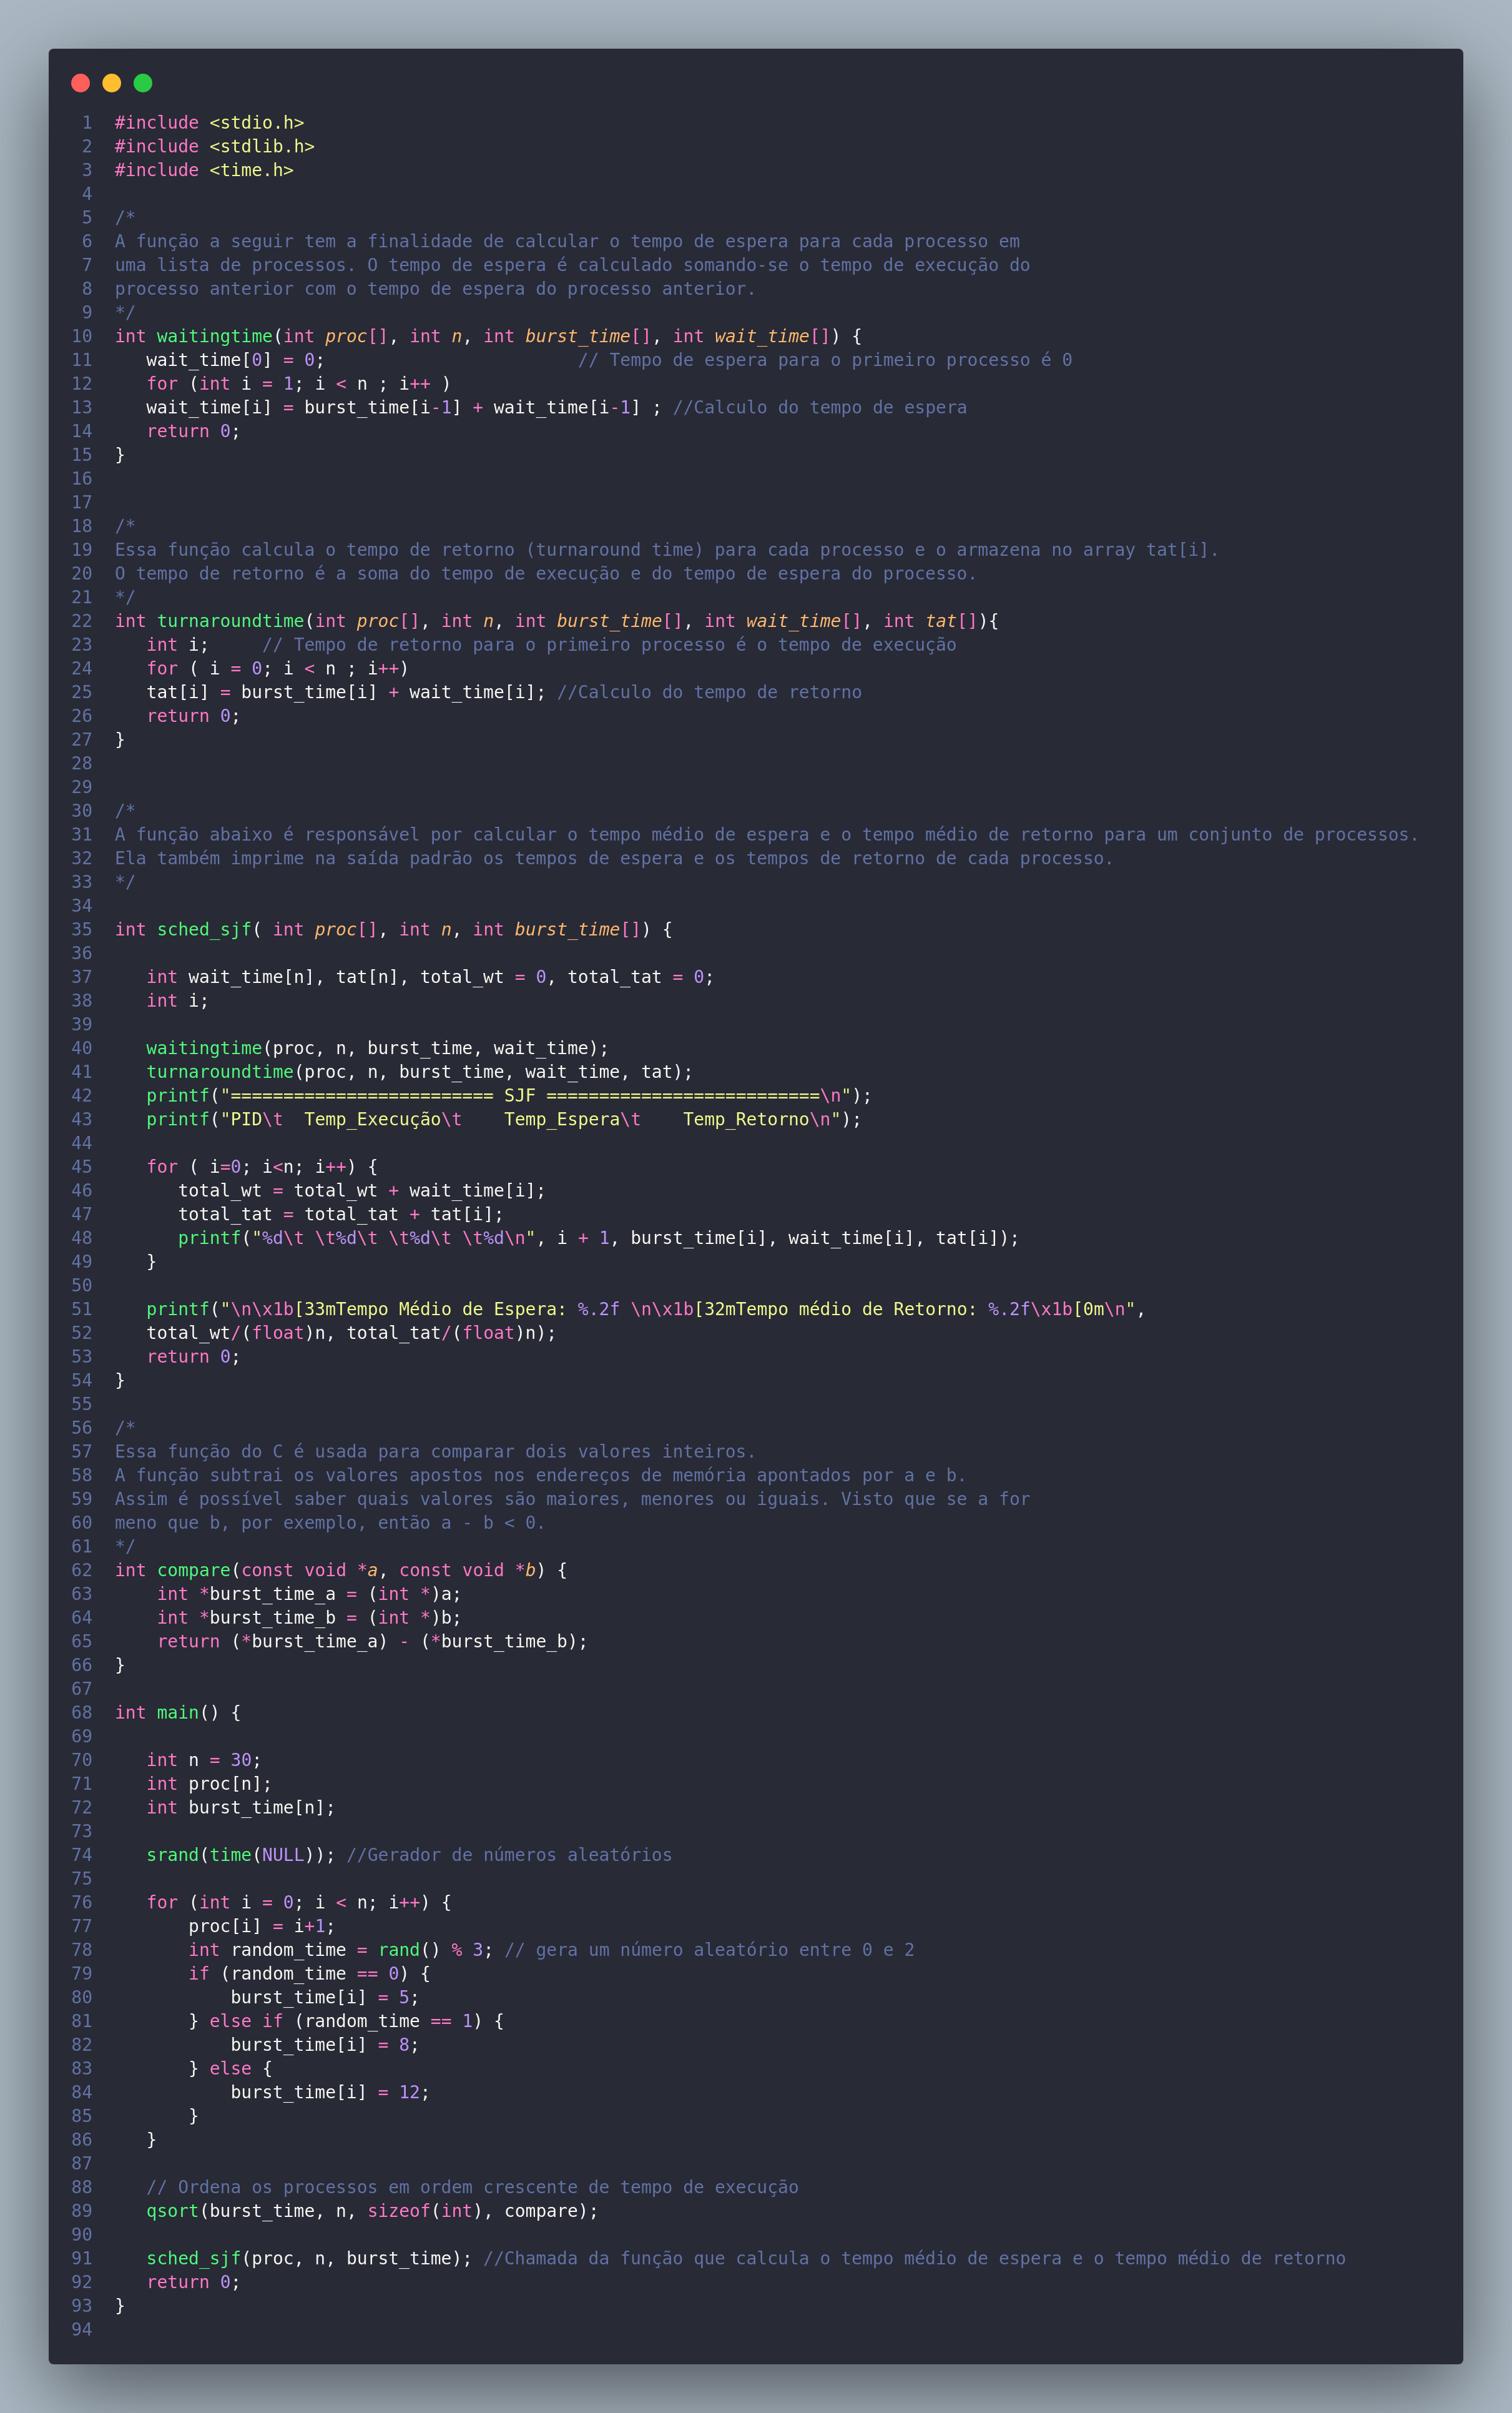
\includegraphics[width=0.6\textwidth]{imagens/sjf_src.png}
    \caption{Código em C. Disponível em: \href{https://github.com/jvictorferreira3301/Sistemas_Operacionais/blob/main/3_escalonadores/sched-sjf.c}{github.com/jvictorferreira3301/SistemasOperacionais/blob/main
    /3\_escalonadores/sched-sjf.c}}
    \label{fig:sjf}
\end{figure}

\begin{figure}[H]
    \centering
    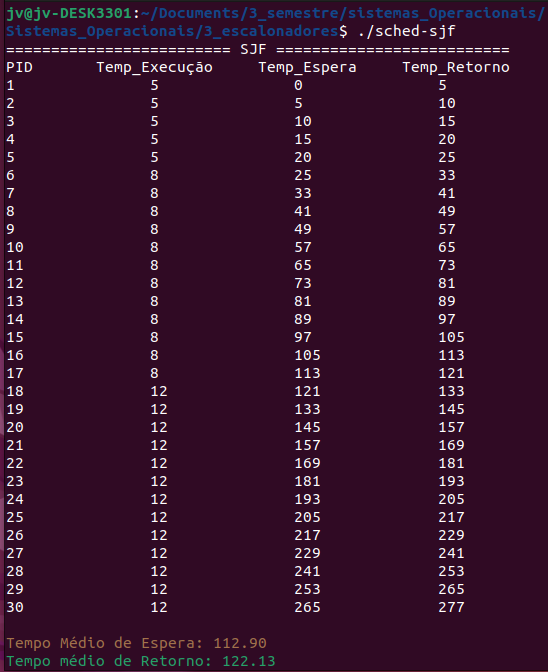
\includegraphics[width=0.7\textwidth]{imagens/sjf_run.png}
    \caption{Execução do Código em C.}
    \label{fig:sjf_run}
\end{figure}

\subsection{Explicação do código}

\begin{itemize}
    \item \textbf{Variáveis-chave:}
      \begin{itemize}
        \item `proc[]`: Um array que representa os identificadores dos processos (PID).
        \item `burst\_time[]`: Um array que armazena o tempo de execução de cada processo.
        \item `wait\_time[]`: Um array para armazenar o tempo de espera de cada processo.
        \item `tat[]`: Um array para armazenar o tempo de retorno (Turnaround\ Time) de cada processo.
        \item `total\_wt`: Variável para rastrear o tempo total de espera de todos os processos.
        \item `total\_tat`: Variável para rastrear o tempo total de retorno de todos os processos.
      \end{itemize}
  
    \item \textbf{Funções:}
      \begin{itemize}
        \item `waitingtime()`: Calcula o tempo de espera para cada processo, somando o tempo de execução do processo anterior com o tempo de espera do processo anterior.
        \item `turnaroundtime()`: Calcula o tempo de retorno para cada processo, que é a soma do tempo de execução e do tempo de espera.
        \item `compare()`: Função de comparação usada para ordenar os processos em ordem crescente de tempo de execução.
      \end{itemize}
  
    \item \textbf{Funcionamento:}
      \begin{itemize}
        \item Inicialmente, os processos são criados com tempos de execução variáveis, que refletem a natureza realista dos processos.
        \item Os processos são então ordenados em ordem crescente com base no tempo de execução. Isso garante que os processos mais curtos sejam agendados primeiro.
        \item O tempo de espera e o tempo de retorno são calculados para cada processo usando as funções `waitingtime()` e `turnaroundtime()`.
        \item Os resultados são impressos, mostrando o PID, o tempo de execução, o tempo de espera e o tempo de retorno de cada processo.
        \item Finalmente, são calculados os tempos médios de espera e de retorno e exibidos na saída.
      \end{itemize}
  \end{itemize}

%%%%%%%%%%%%%%%%%%%%%%%%%%%%%%%%%%%%%%%%%%%%%%%%%%%%%%%%%%%%%%%%%%%%%%%%%%%%%%%%%%%%%%%%%%%%%%

\section{Algoritmo SRTF (Shortest Remaining Time First)}
Nesta seção, abordaremos a implementação do algoritmo de escalonamento SRTF 
(Shortest Remaining Time First), que tem como objetivo agendar processos com base no tempo 
de execução mais curto. Essa abordagem é eficaz na minimização do tempo de espera 
dos processos e na melhoria do desempenho do sistema de escalonamento. 

Na figura \ref{fig:srtf} é evidenciada a implementação desse algoritmo e posteriormente, na figura \ref{fig:srtf_run},
a execução do mesmo seguida da explicação do código.

\begin{figure}[H]
    \centering
    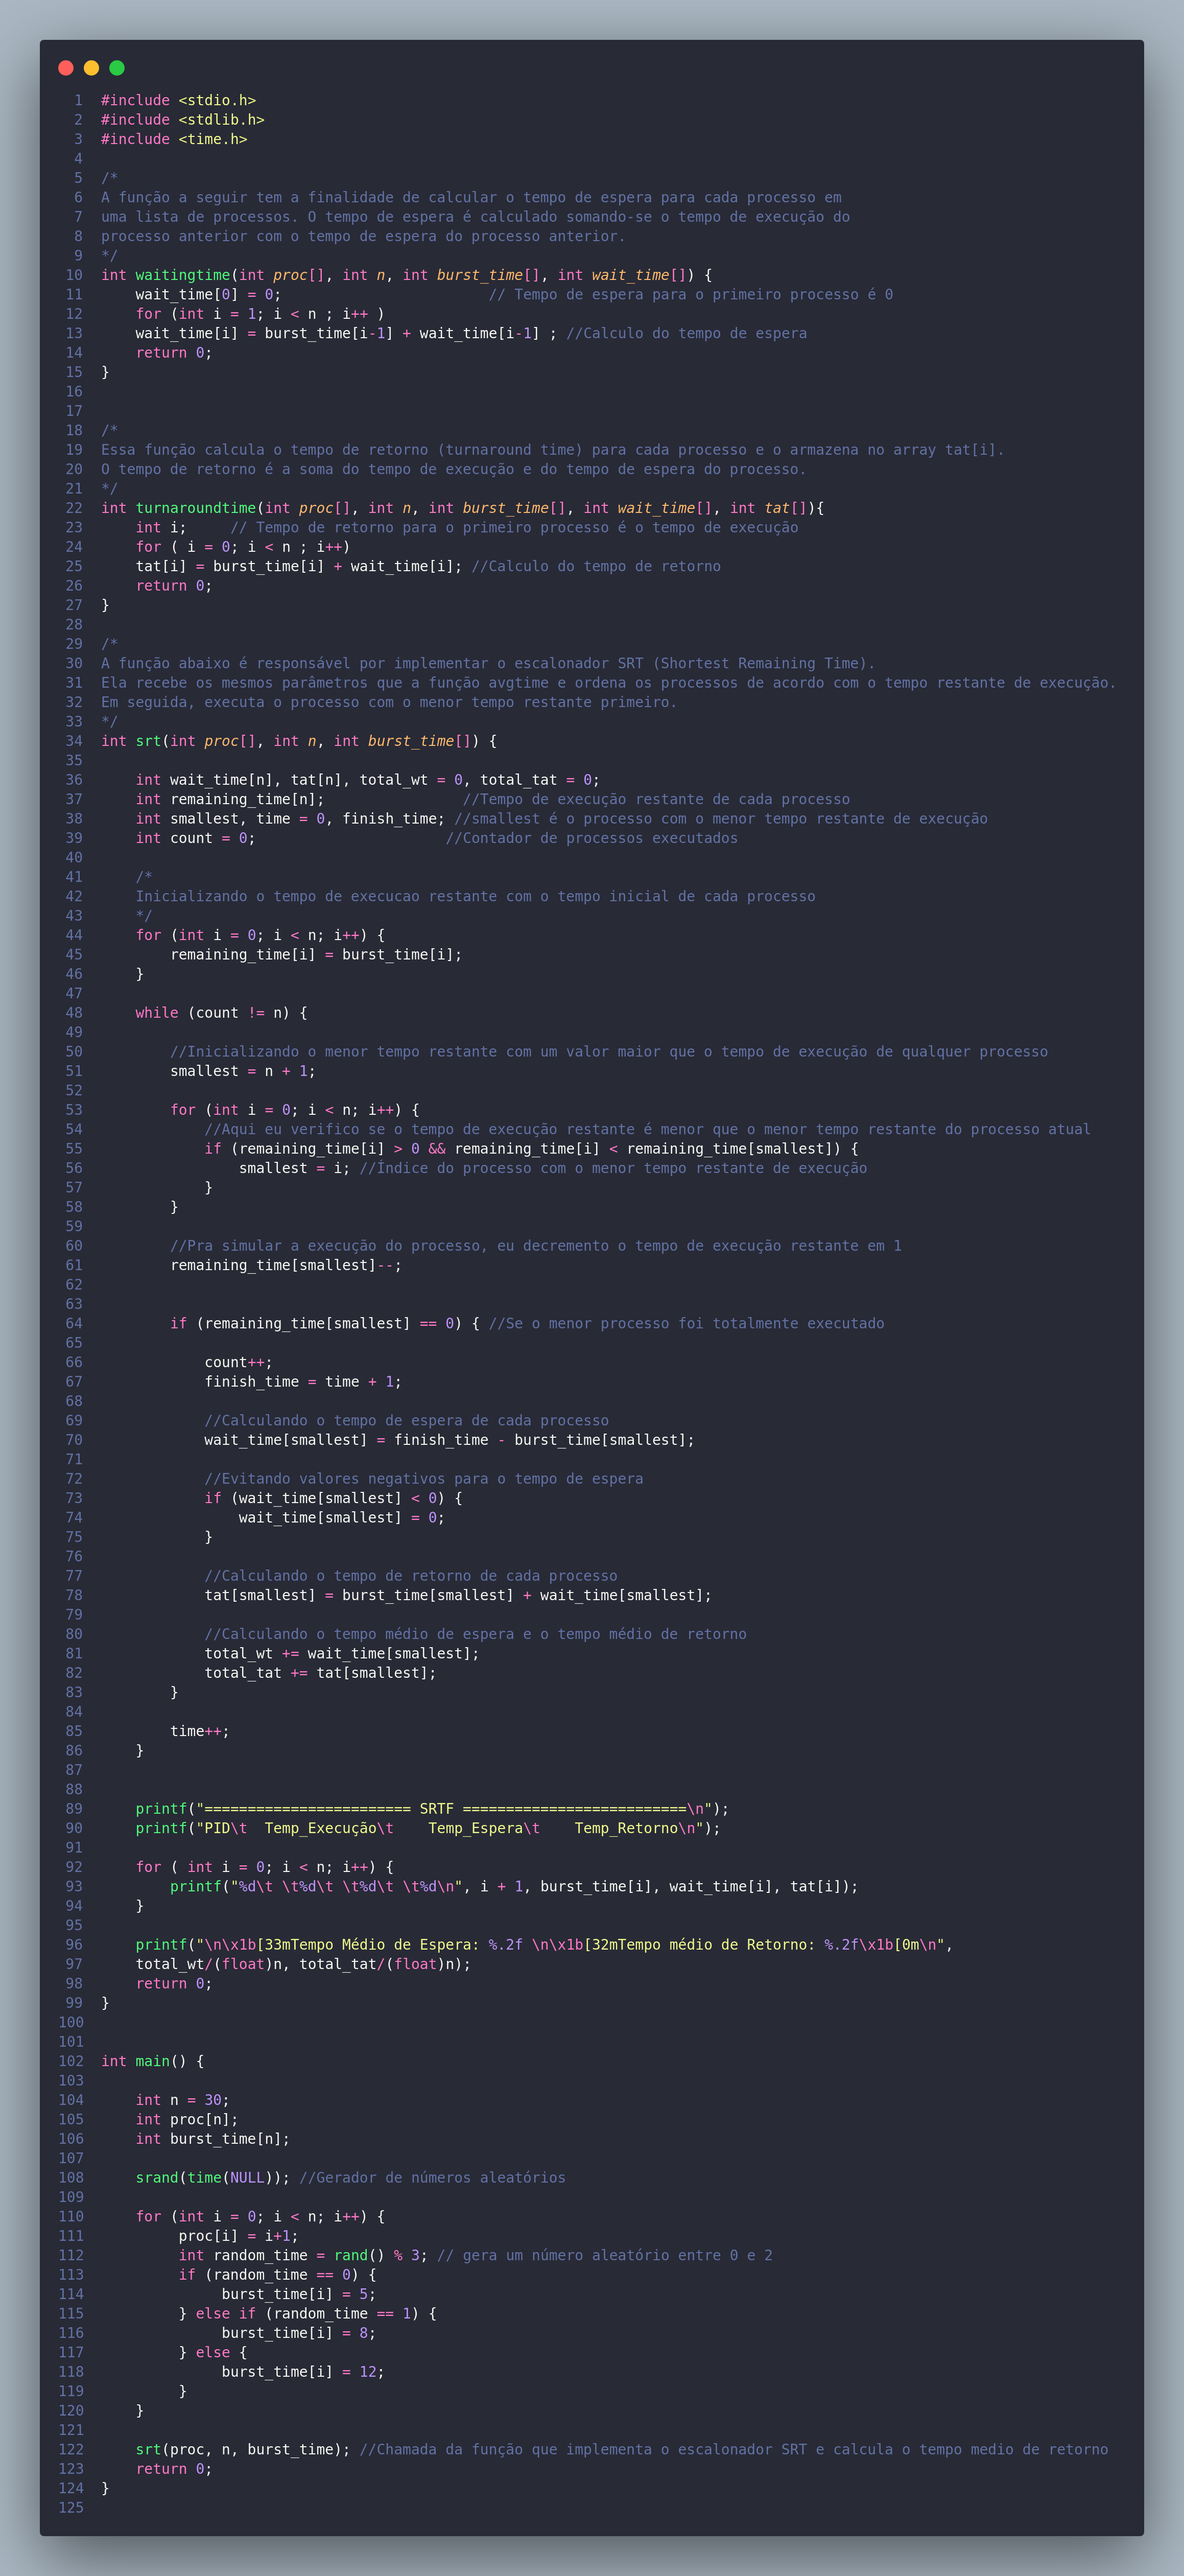
\includegraphics[width=0.7\textwidth]{imagens/srtf_src.png}
    \caption{Código em C. Disponível em: \href{https://github.com/jvictorferreira3301/Sistemas_Operacionais/blob/main/3_escalonadores/sched-srtf.c}{github.com/jvictorferreira3301/SistemasOperacionais/blob/main/
    3\_escalonadores/sched-srtf.c}}
    \label{fig:srtf}
\end{figure}

\begin{figure}[H]
    \centering
    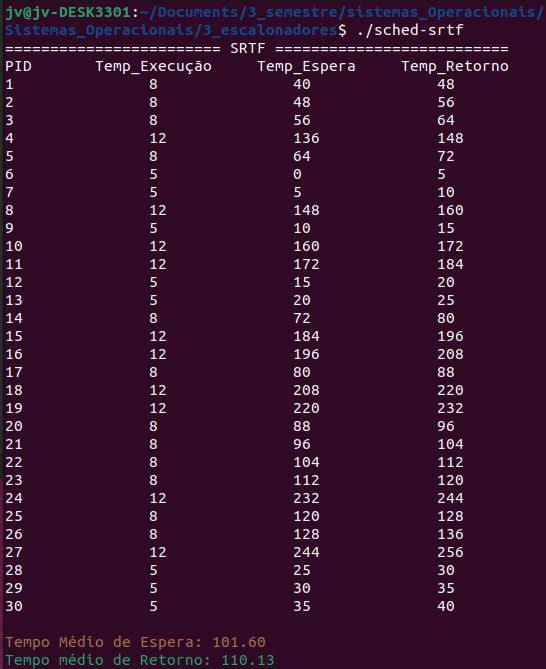
\includegraphics[width=0.7\textwidth]{imagens/srtf_run.png}
    \caption{Execução do Código em C.}
    \label{fig:srtf_run}
\end{figure}

\subsection{Explicação do código}

\begin{itemize}
    \item \textbf{Variáveis-chave:}
      \begin{itemize}
        \item `proc[]`: Um array que representa os identificadores dos processos (PID).
        \item `burst\_time[]`: Um array que armazena o tempo de execução de cada processo.
        \item `wait\_time[]`: Um array para armazenar o tempo de espera de cada processo.
        \item `tat[]`: Um array para armazenar o tempo de retorno (Turnaround\ Time) de cada processo.
        \item `total\_wt`: Variável para rastrear o tempo total de espera de todos os processos.
        \item `total\_tat`: Variável para rastrear o tempo total de retorno de todos os processos.
      \end{itemize}
  
    \item \textbf{Funções:}
      \begin{itemize}
        \item `waitingtime()`: Calcula o tempo de espera para cada processo, somando o tempo de execução do processo anterior com o tempo de espera do processo anterior.
        \item `turnaroundtime()`: Calcula o tempo de retorno para cada processo, que é a soma do tempo de execução e do tempo de espera.
        \item `srt()`: Função que implementa o escalonador SRTF (Shortest Remaining Time First) e ordena os processos de acordo com o tempo restante de execução. Ela também calcula o tempo médio de espera e de retorno.
      \end{itemize}
  
    \item \textbf{Funcionamento:}
      \begin{itemize}
        \item Inicialmente, os processos são criados com tempos de execução variáveis, que refletem a natureza realista dos processos.
        \item O algoritmo SRTF executa os processos com o menor tempo de execução restante, priorizando os processos mais curtos.
        \item O tempo de espera e o tempo de retorno são calculados para cada processo usando as funções `waitingtime()` e `turnaroundtime()`.
        \item Os resultados são impressos, mostrando o PID, o tempo de execução, o tempo de espera e o tempo de retorno de cada processo.
        \item Finalmente, são calculados os tempos médios de espera e de retorno e exibidos na saída.
      \end{itemize}
  \end{itemize}

%%%%%%%%%%%%%%%%%%%%%%%%%%%%%%%%%%%%%%%%%%%%%%%%%%%%%%%%%%%%%%%%%%%%%%%%%%%%%%%%%%%%%%%%%%%%%%

\section{Algoritmo de Prioridades}
Nesta seção, apresentaremos a implementação do algoritmo de escalonamento de prioridades. 
Este algoritmo tem como objetivo agendar processos com base em prioridades atribuídas a cada processo. 
A ideia fundamental é que processos com prioridades mais altas têm preferência para execução em relação 
aos processos com prioridades mais baixas. O escalonador escolherá o processo com a prioridade mais alta 
para execução. Esse algoritmo permite que processos críticos ou importantes sejam atendidos prontamente, 
melhorando o desempenho e a eficiência do sistema de escalonamento de processos.

O código C na figura \ref{fig:prioridades} demonstra a implementação do algoritmo 
de prioridades, e a figura \ref{fig:prioridades_run} mostra sua execução.

\begin{figure}[H]
    \centering
    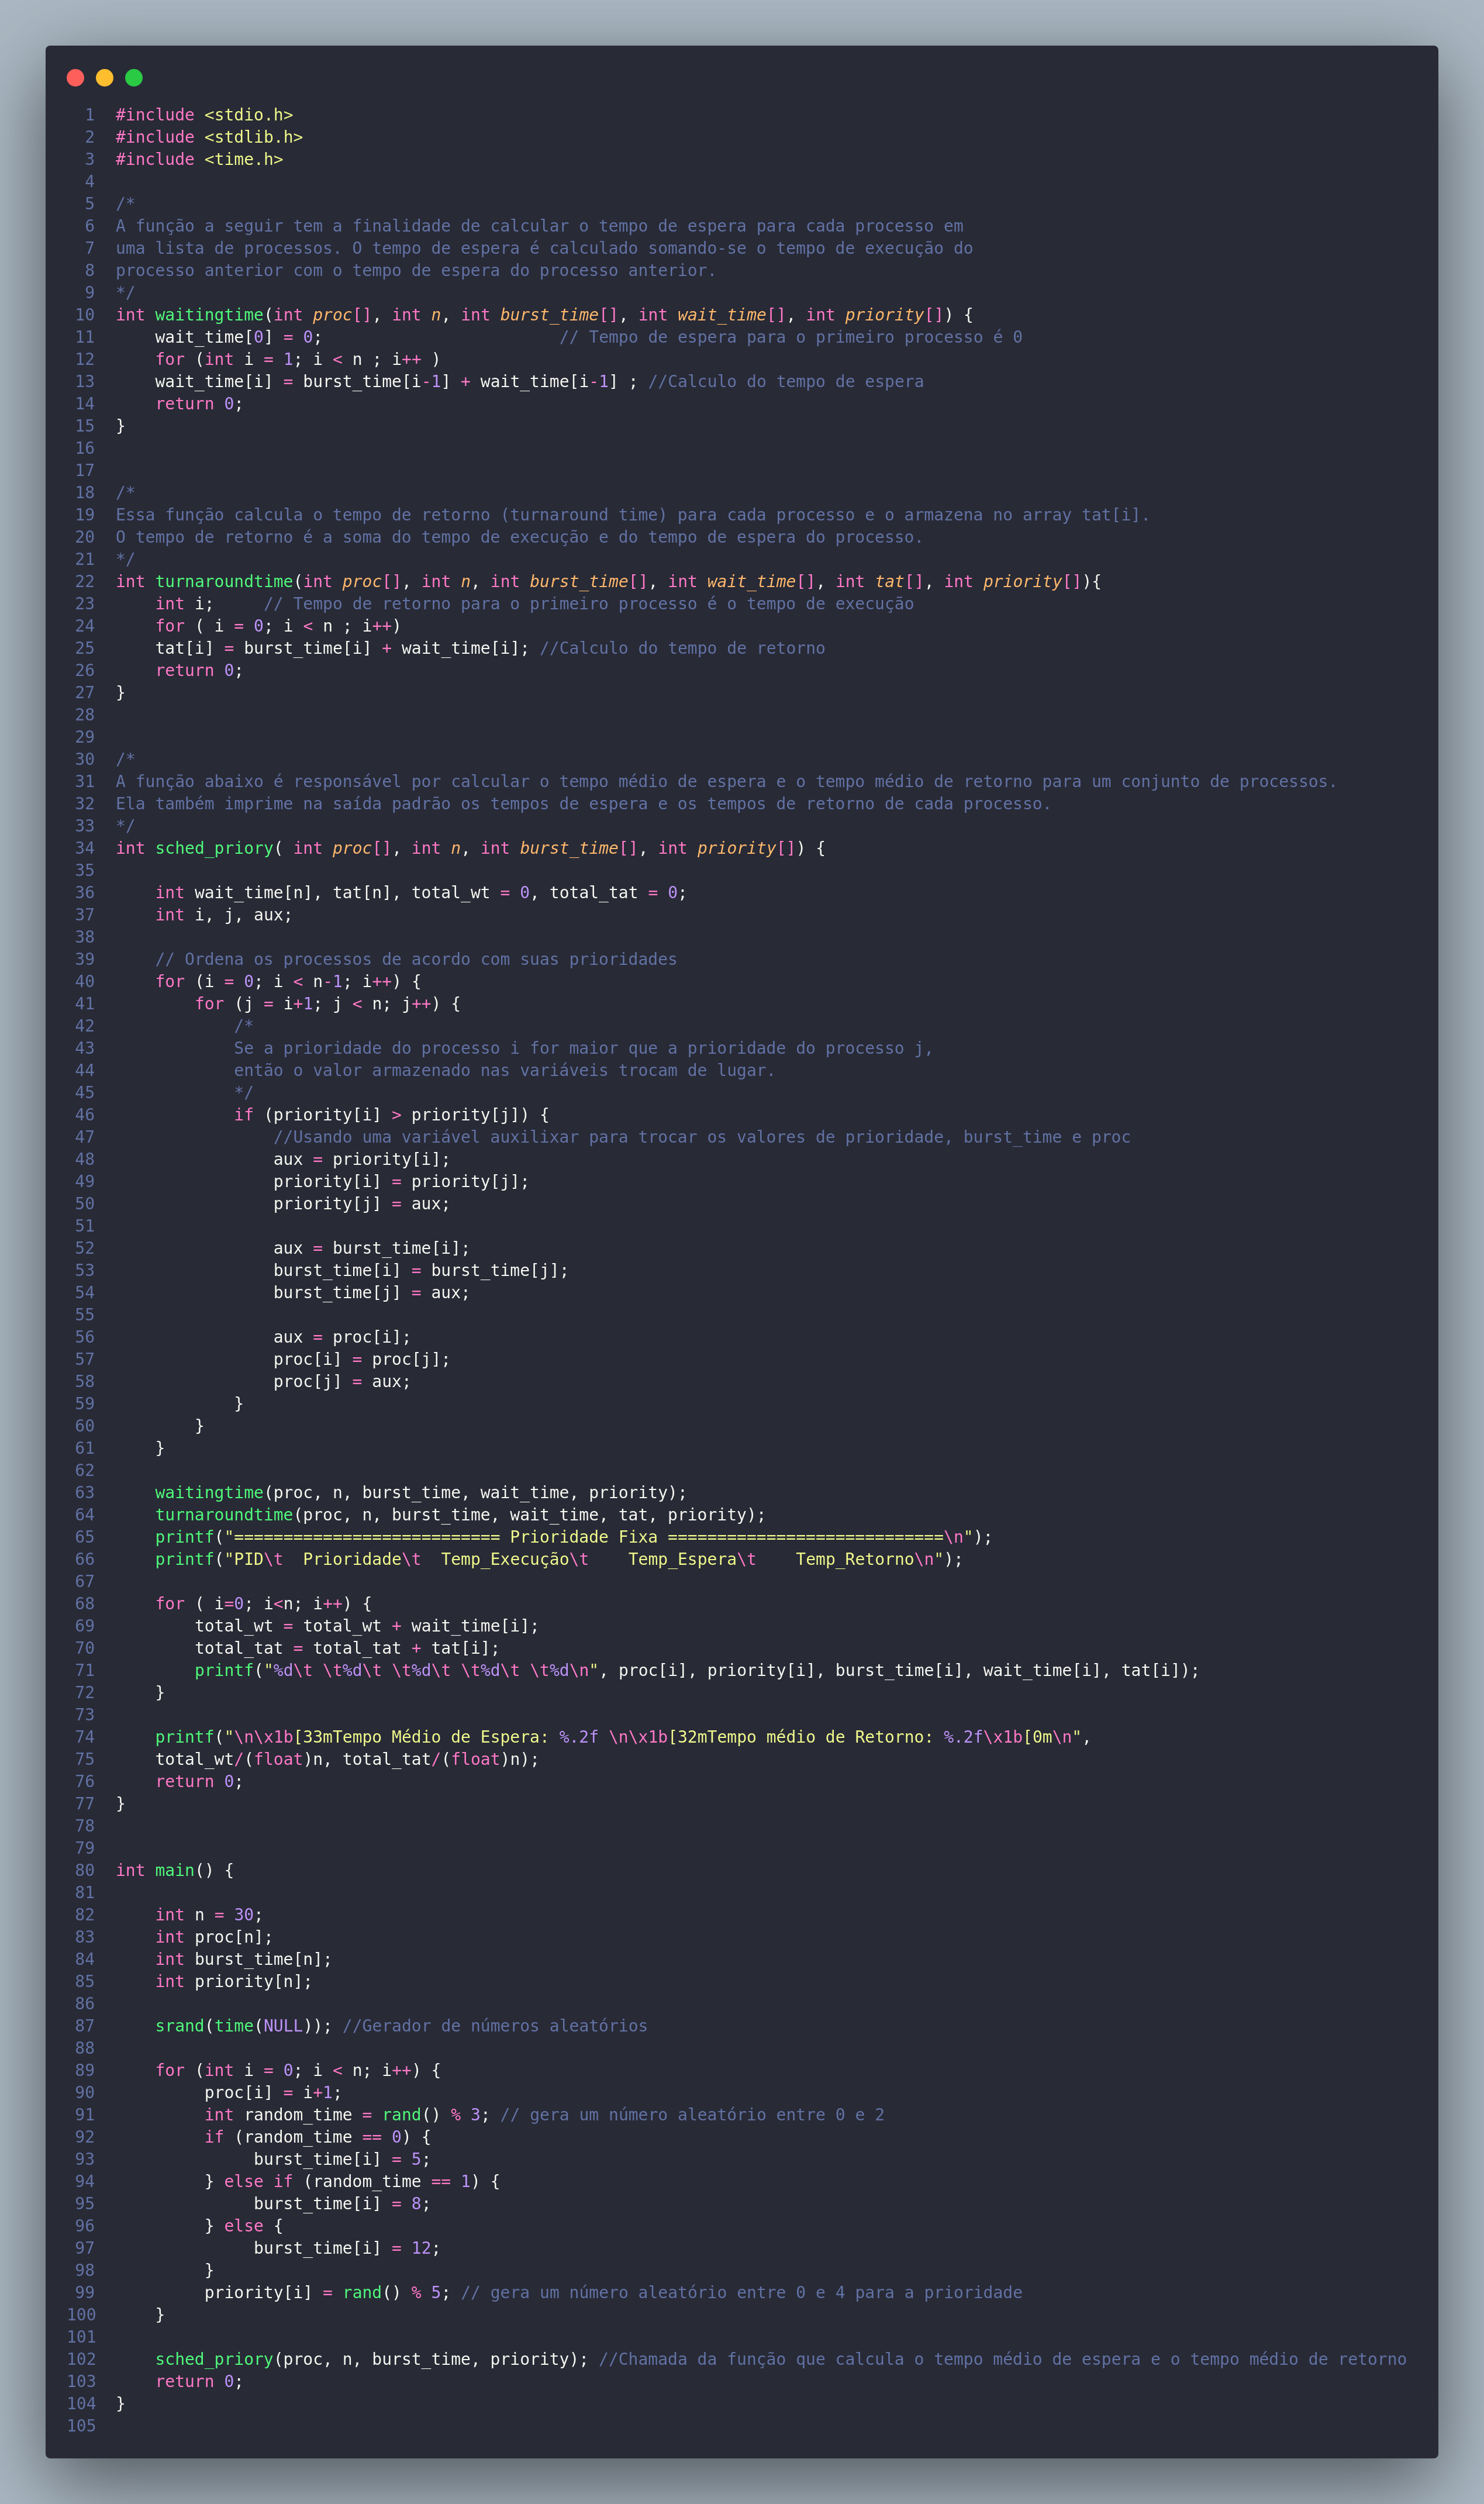
\includegraphics[width=0.9\textwidth]{imagens/prioridades_src.png}
    \caption{Código em C. Disponível em: \href{https://github.com/jvictorferreira3301/Sistemas_Operacionais/blob/main/3_escalonadores/sched-prioridades.c}{github.com/jvictorferreira3301/SistemasOperacionais/blob/main/
    3\_escalonadores/sched-prioridades.c}}
    \label{fig:prioridades}
\end{figure}

\begin{figure}[H]
    \centering
    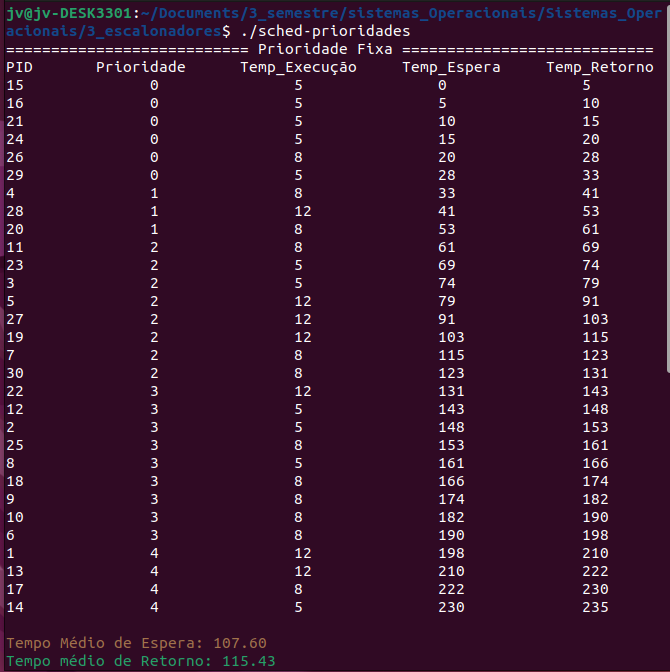
\includegraphics[width=0.7\textwidth]{imagens/prioridades_run.png}
    \caption{Execução do Código em C.}
    \label{fig:prioridades_run}
\end{figure}

\subsection{Explicação do código}

\begin{itemize}
    \item \textbf{Variáveis-chave:}
      \begin{itemize}
        \item `proc[]`: Um array que representa os identificadores dos processos (PID).
        \item `burst\_time[]`: Um array que armazena o tempo de execução de cada processo.
        \item `wait\_time[]`: Um array para armazenar o tempo de espera de cada processo.
        \item `tat[]`: Um array para armazenar o tempo de retorno (Turnaround\ Time) de cada processo.
        \item `priority[]`: Um array que representa a prioridade de cada processo.
        \item `total\_wt`: Variável para rastrear o tempo total de espera de todos os processos.
        \item `total\_tat`: Variável para rastrear o tempo total de retorno de todos os processos.
      \end{itemize}
  
    \item \textbf{Funções:}
      \begin{itemize}
        \item `waitingtime()`: Calcula o tempo de espera para cada processo, somando o tempo de execução do processo anterior com o tempo de espera do processo anterior.
        \item `turnaroundtime()`: Calcula o tempo de retorno para cada processo, que é a soma do tempo de execução e do tempo de espera.
        \item `sched\_priory()`: Função principal que implementa o algoritmo de prioridades, ordena os processos com base em suas prioridades e calcula os tempos de espera e de retorno.
      \end{itemize}
  
    \item \textbf{Funcionamento:}
      \begin{itemize}
        \item Inicialmente, os processos são criados com tempos de execução e prioridades variáveis, refletindo cenários realistas.
        \item Os processos são ordenados em ordem crescente de prioridade.
        \item O tempo de espera e o tempo de retorno são calculados para cada processo usando as funções `waitingtime()` e `turnaroundtime()`.
        \item Os resultados são impressos, mostrando o PID, a prioridade, o tempo de execução, o tempo de espera e o tempo de retorno de cada processo.
        \item Finalmente, são calculados os tempos médios de espera e de retorno e exibidos na saída.
      \end{itemize}
  \end{itemize}
%%%%%%%%%%%%%%%%%%%%%%%%%%%%%%%%%%%%%%%%%%%%%%%%%%%%%%%%%%%%%%%%%%%%%%%%%%%%%%%%%%%%%%%%%%%%%%

\section{Algoritmo Round Robin}
Nesta seção, apresentaremos a implementação do algoritmo de escalonamento Round Robin.que tem como
objetivo agendar processos de maneira equitativa, alocando uma fatia de tempo igual para cada processo 
na fila de prontos. O Round Robin é conhecido por sua abordagem justa e eficaz na prevenção de inanição 
de processos. Ele oferece uma alocação de tempo de CPU equitativa a todos os processos, o 
que é fundamental para garantir que nenhum processo monopolize os recursos e que todos tenham 
a oportunidade de serem executados. Isso é particularmente útil em ambientes multiusuários, 
onde diversos processos concorrem por recursos de computação.  

O código C na figura \ref{fig:rr} demonstra a implementação do algoritmo Round Robin e 
execução é exposta na figura \ref{fig:rrun}.

\begin{figure}[H]
    \centering
    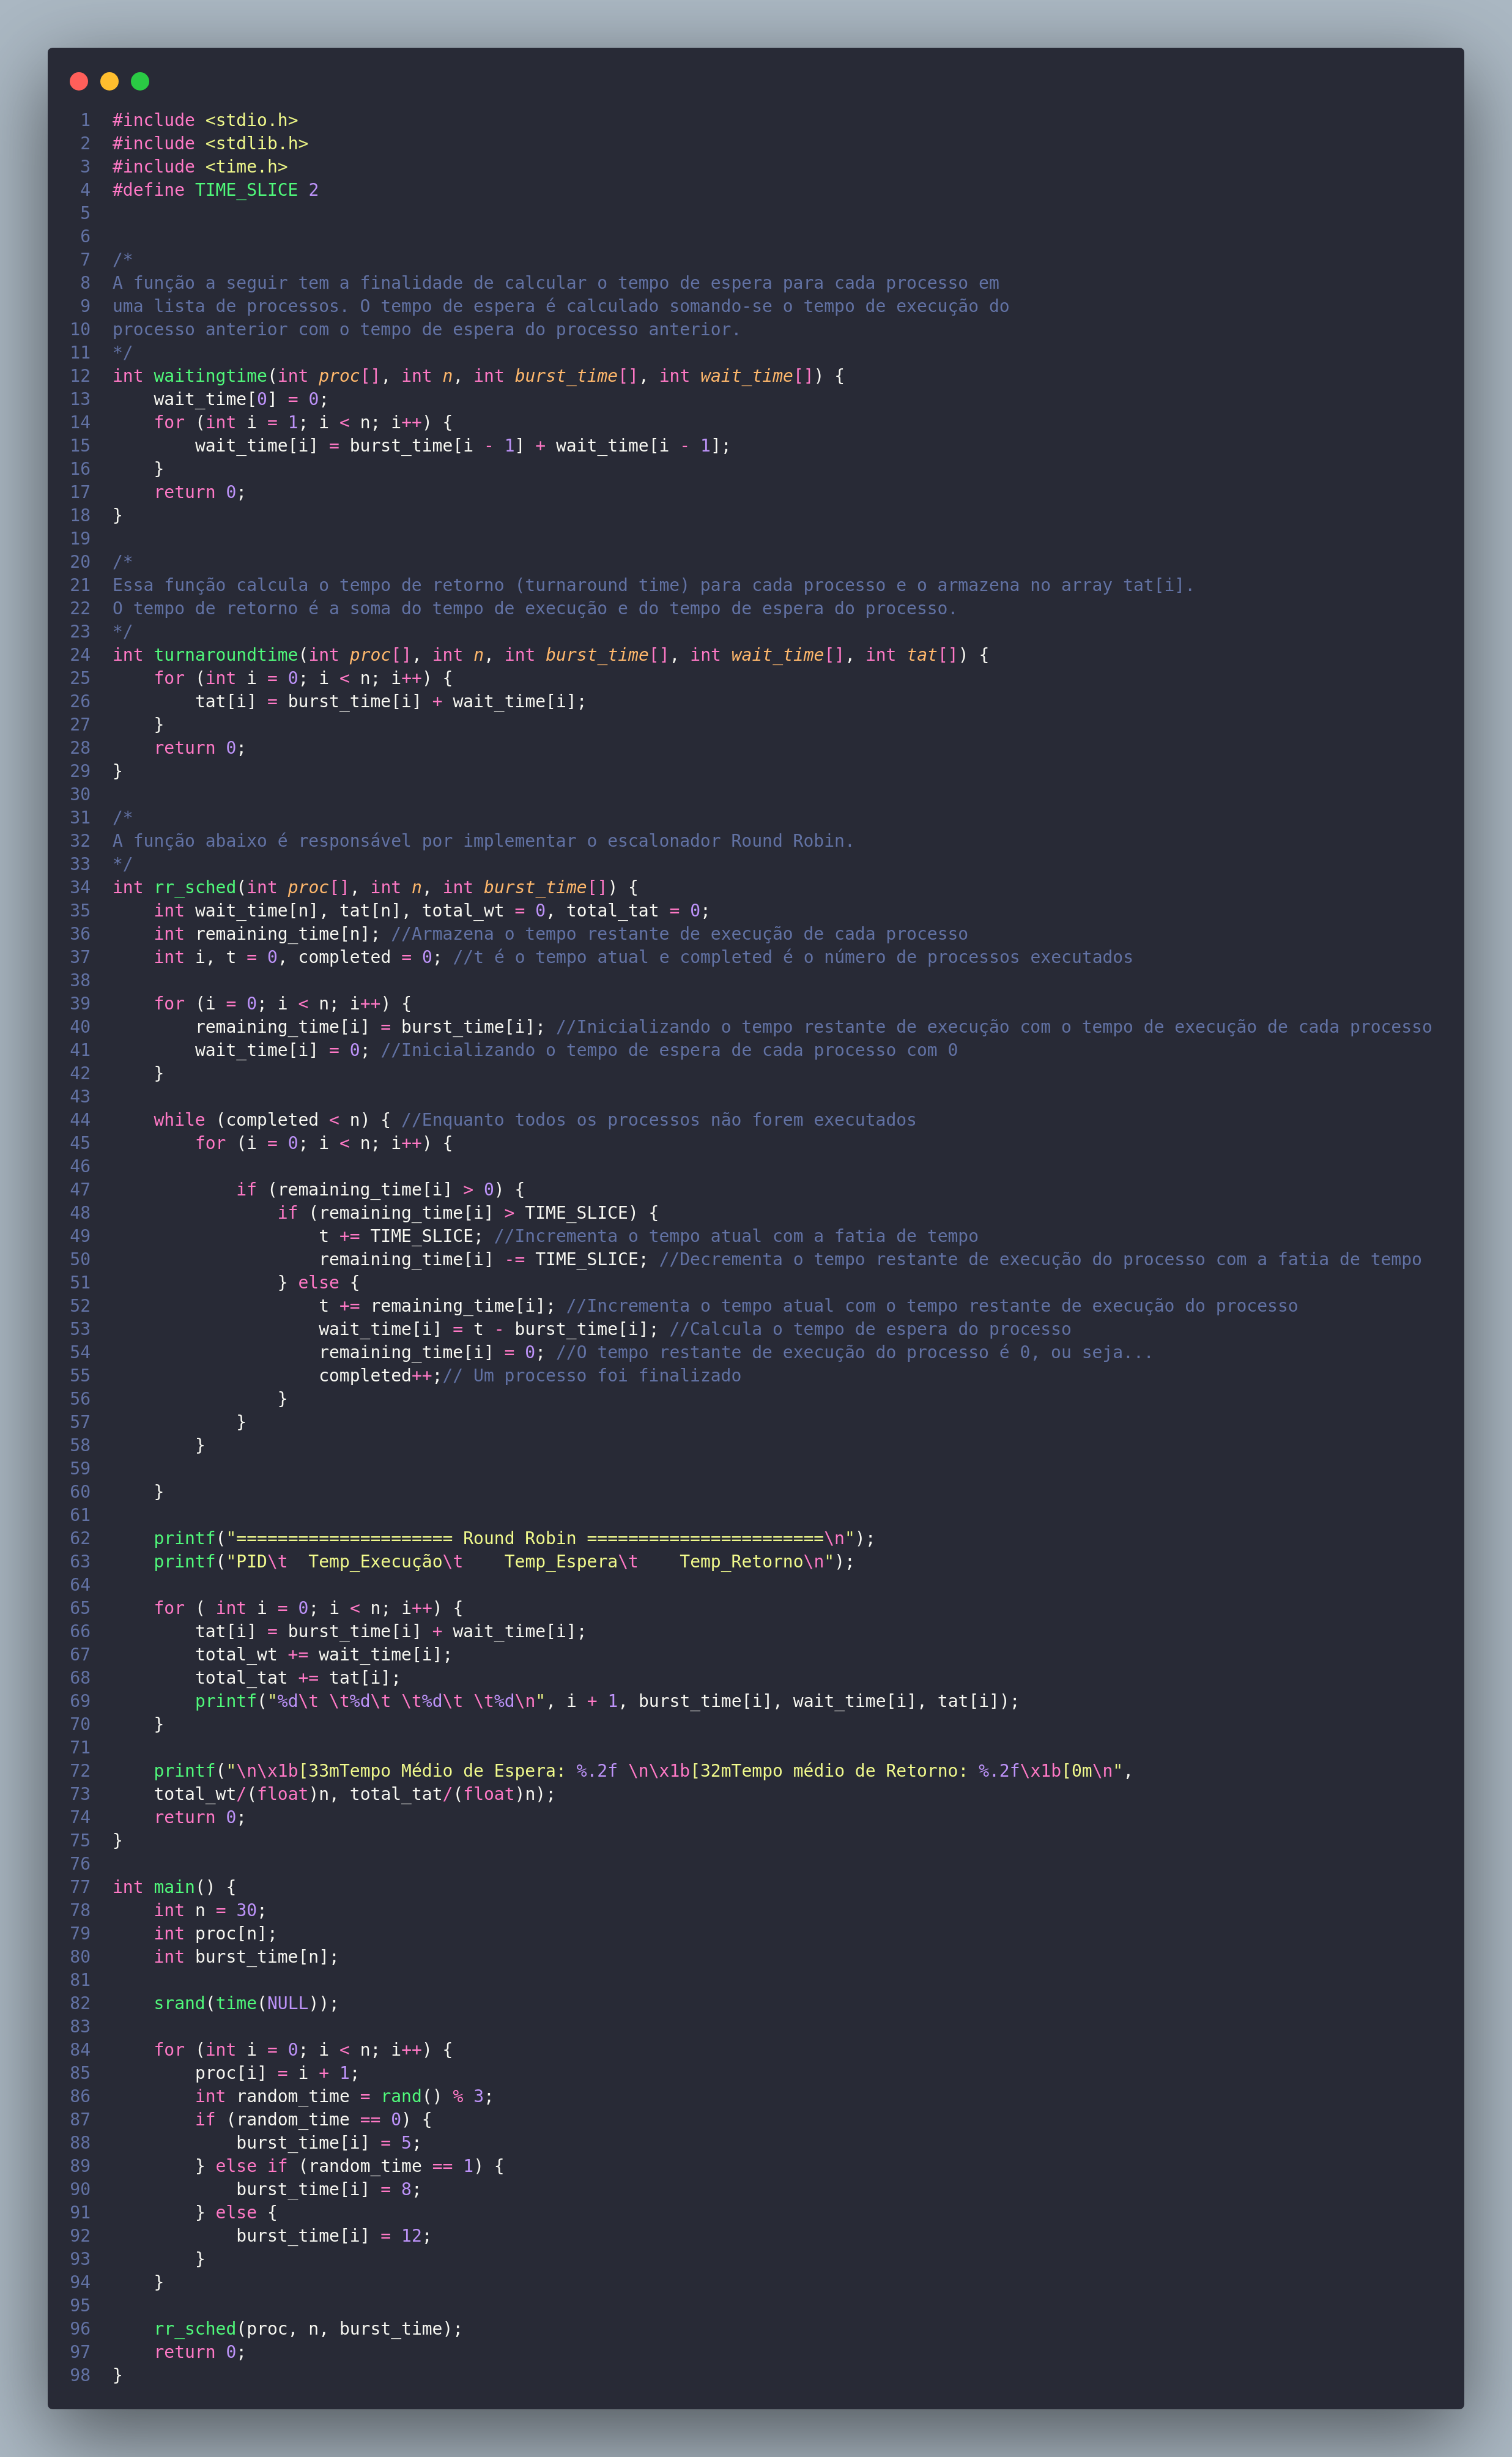
\includegraphics[width=0.9\textwidth]{imagens/rr_src.png}
    \caption{Código em C. Disponível em: \href{https://github.com/jvictorferreira3301/Sistemas_Operacionais/blob/main/3_escalonadores/sched-rr.c}{github.com/jvictorferreira3301/SistemasOperacionais/blob/main/
    3\_escalonadores/sched-rr.c}}
    \label{fig:rr}
\end{figure}

\begin{figure}[H]
    \centering
    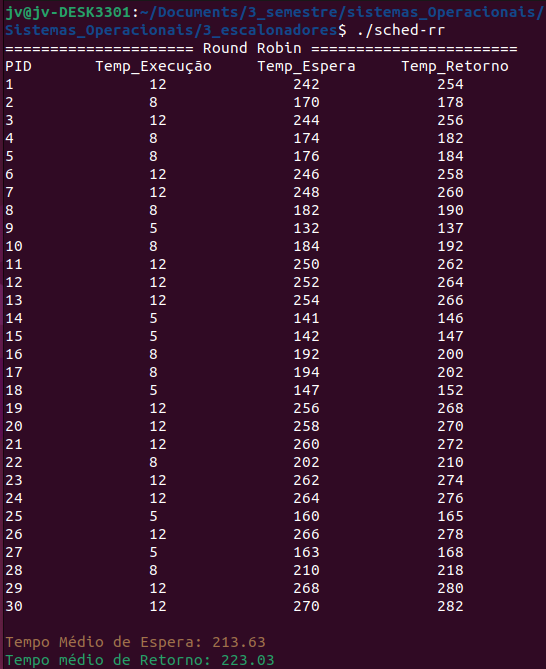
\includegraphics[width=0.7\textwidth]{imagens/rr_run.png}
    \caption{Execução do Código em C.}
    \label{fig:rrun}
\end{figure}

\subsection{Explicação do código}

\begin{itemize}
    \item \textbf{Variáveis-chave:}
      \begin{itemize}
        \item `proc[]`: Um array que representa os identificadores dos processos (PID).
        \item `burst\_time[]`: Um array que armazena o tempo de execução de cada processo.
        \item `wait\_time[]`: Um array para armazenar o tempo de espera de cada processo.
        \item `tat[]`: Um array para armazenar o tempo de retorno (Turnaround\ Time) de cada processo.
        \item `total\_wt`: Variável para rastrear o tempo total de espera de todos os processos.
        \item `total\_tat`: Variável para rastrear o tempo total de retorno de todos os processos.
      \end{itemize}
  
    \item \textbf{Funções:}
      \begin{itemize}
        \item `waitingtime()`: Calcula o tempo de espera para cada processo, somando o tempo de execução do processo anterior com o tempo de espera do processo anterior.
        \item `turnaroundtime()`: Calcula o tempo de retorno para cada processo, que é a soma do tempo de execução e do tempo de espera.
      \end{itemize}
  
    \item \textbf{Funcionamento:}
      \begin{itemize}
        \item Inicialmente, os processos são criados com tempos de execução variáveis, que refletem a natureza realista dos processos.
        \item O algoritmo Round Robin atribui a cada processo um "time-slice" fixo definido como \textbf{TIME\_SLICE}.
        \item Os processos são executados de acordo com o Round Robin, onde cada processo é executado por um período de tempo, após o qual é colocado de volta na fila e o próximo processo é executado.
        \item O tempo de espera e o tempo de retorno são calculados para cada processo usando as funções `waitingtime()` e `turnaroundtime()`.
        \item Os resultados são impressos, mostrando o PID, o tempo de execução, o tempo de espera e o tempo de retorno de cada processo.
        \item Finalmente, são calculados os tempos médios de espera e de retorno e exibidos na saída.
      \end{itemize}
  \end{itemize}
%%%%%%%%%%%%%%%%%%%%%%
%%%%%%%%%%%%%%%%%%%%%%%%%%%%%%%%%%%%%%%%%%%%%%%%%%%%%%%%%%%%%%%%%%%%%%%%%%%%%%%%%%%%%%%%

\section{Algoritmo FCFS (First-Come, First-Served)}

Nesta seção, apresentaremos a implementação do algoritmo de escalonamento FCFS. O algoritmo FCFS 
opera com o princípio de que os processos são atendidos na ordem em que chegam à fila de prontidão. 
Ou seja, o primeiro processo que entra na fila é o primeiro a ser executado. Isso torna o FCFS 
um algoritmo de escalonamento simples, mas não necessariamente eficiente em todos os cenários.

O código C na figura \ref{fig:fifo} demonstra a implementação do algoritmo FCFS, e a figura \ref{fig:fifo_run} mostra sua execução.

\begin{figure}[H]
    \centering
    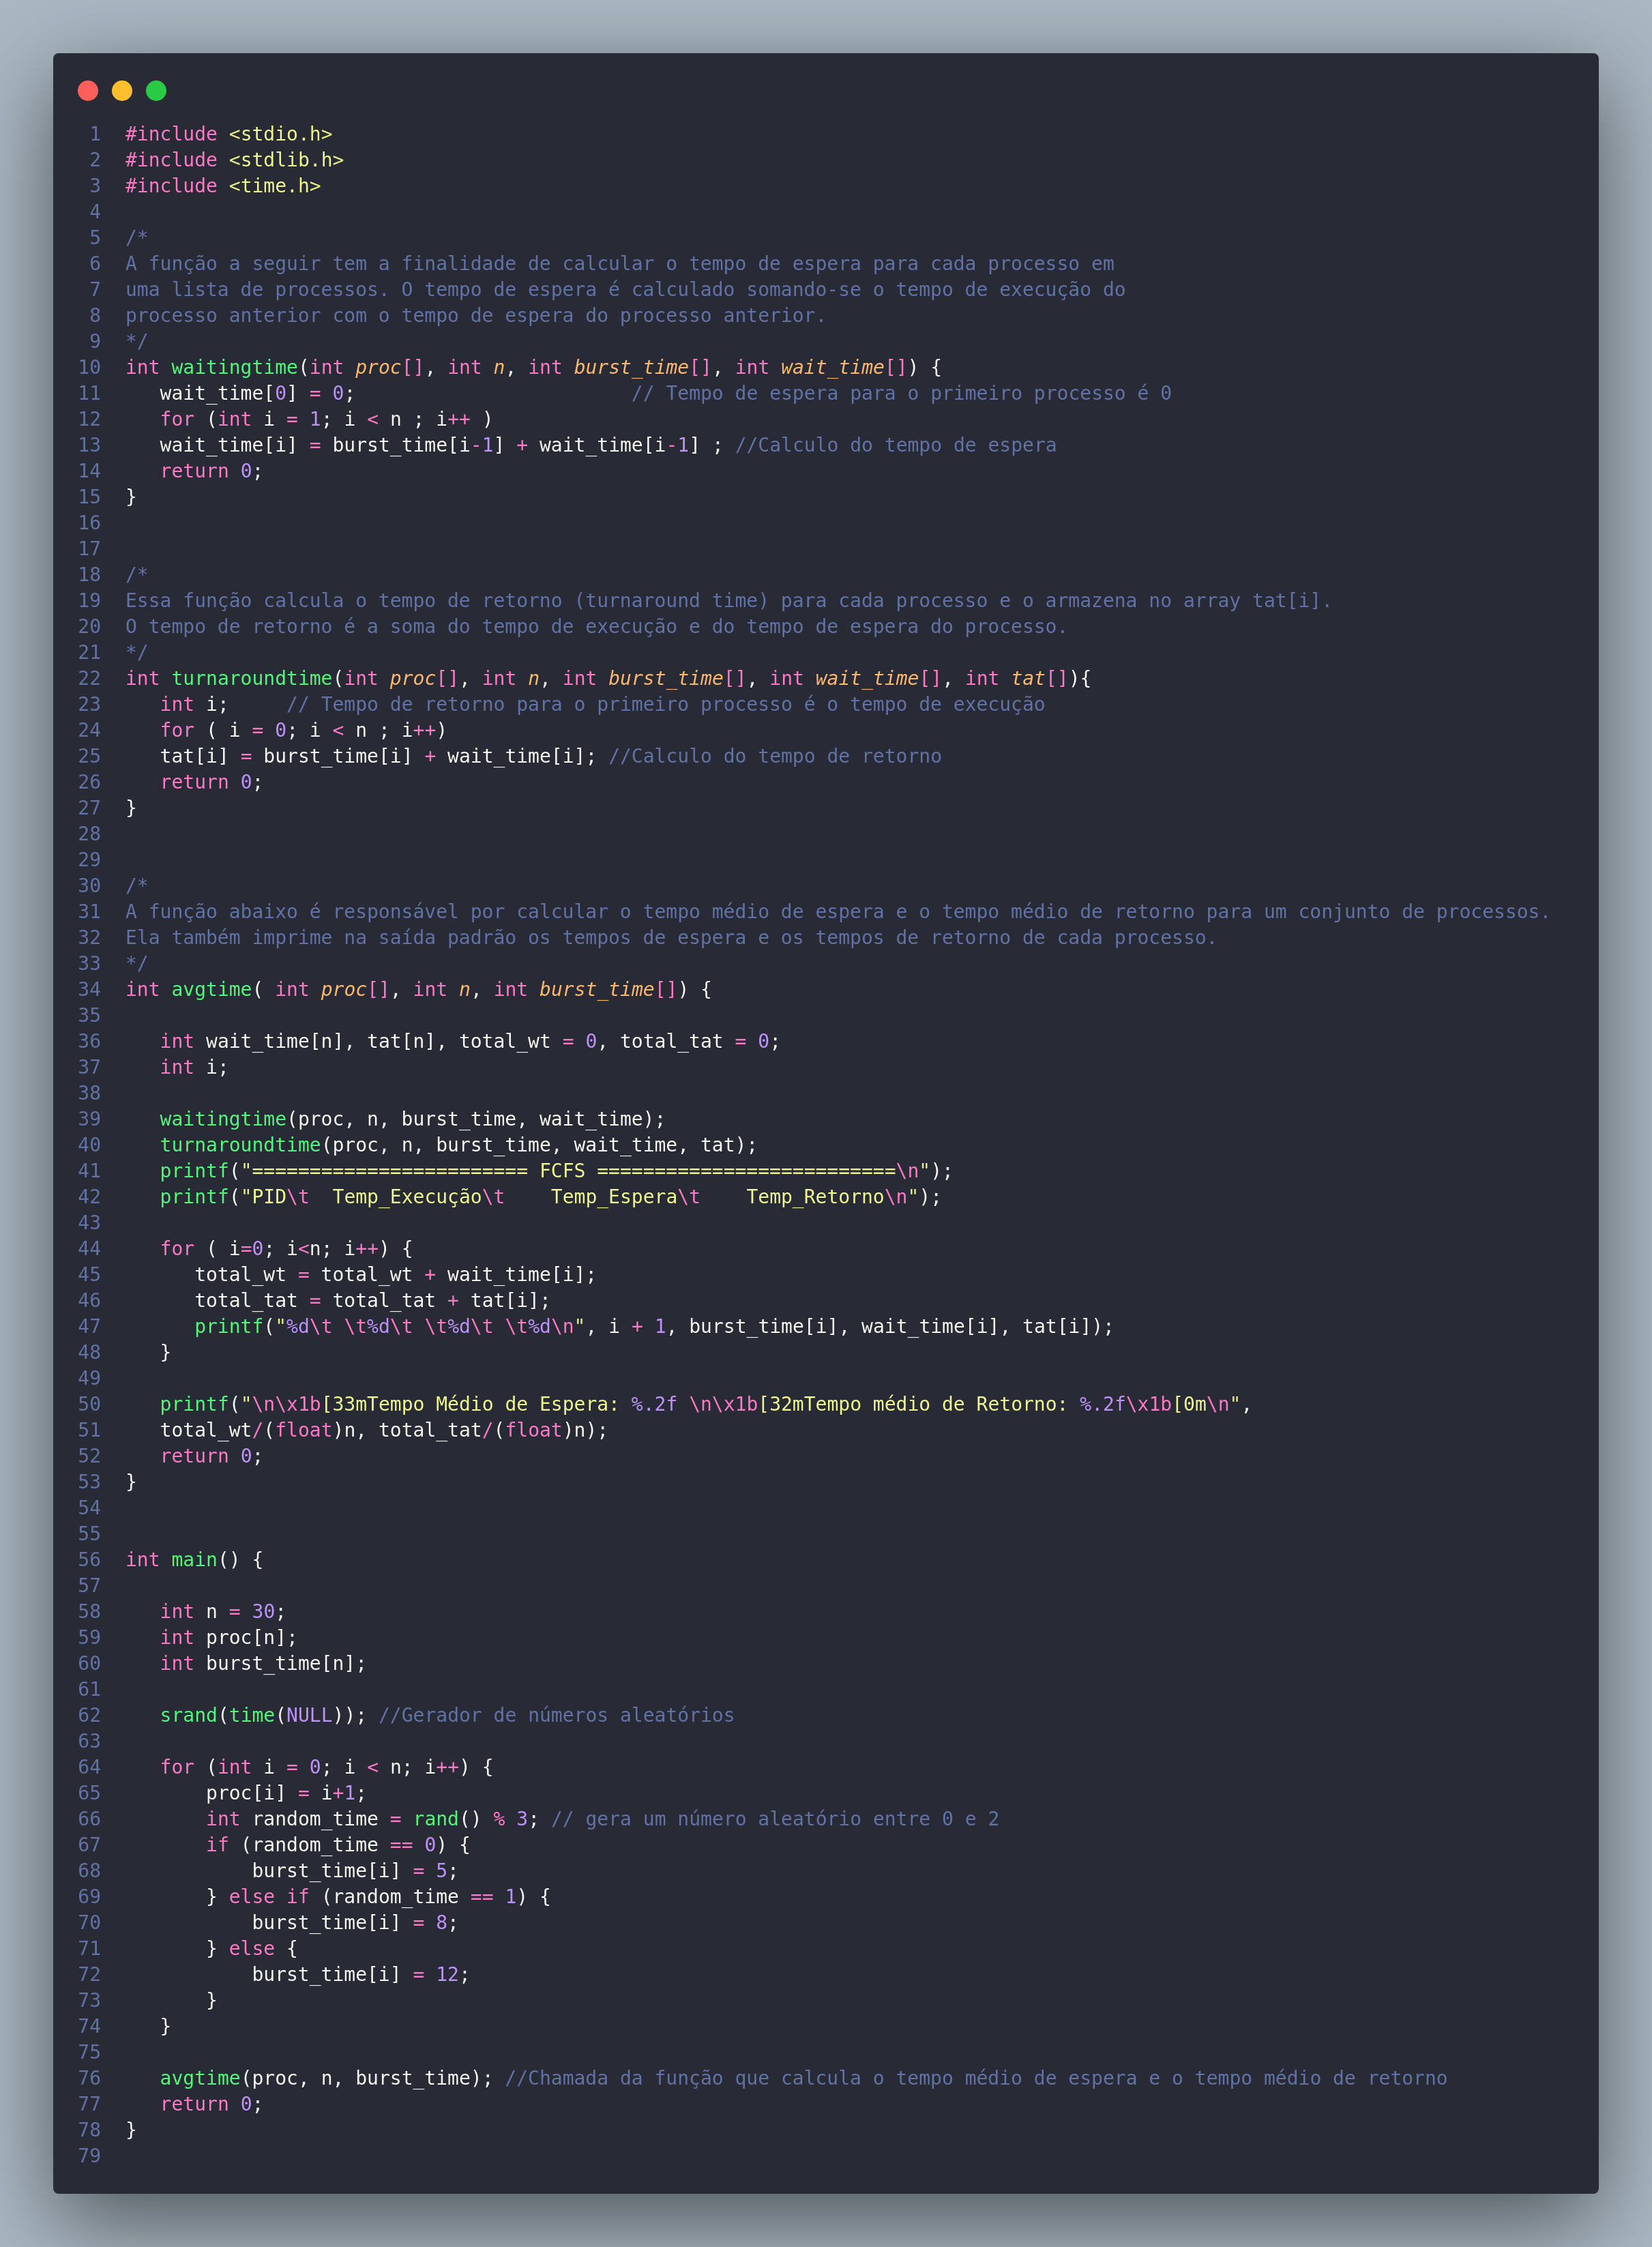
\includegraphics[width=1.1\textwidth]{imagens/fifo_src.png}
    \caption{Código em C. Disponível em: \href{https://github.com/jvictorferreira3301/Sistemas_Operacionais/blob/main/3_escalonadores/sched-fcfs.c}{github.com/jvictorferreira3301/SistemasOperacionais/blob/main/ 3\_escalonadores/sched-fcfs.c}}
    \label{fig:fifo}
\end{figure}

\begin{figure}[H]
    \centering
    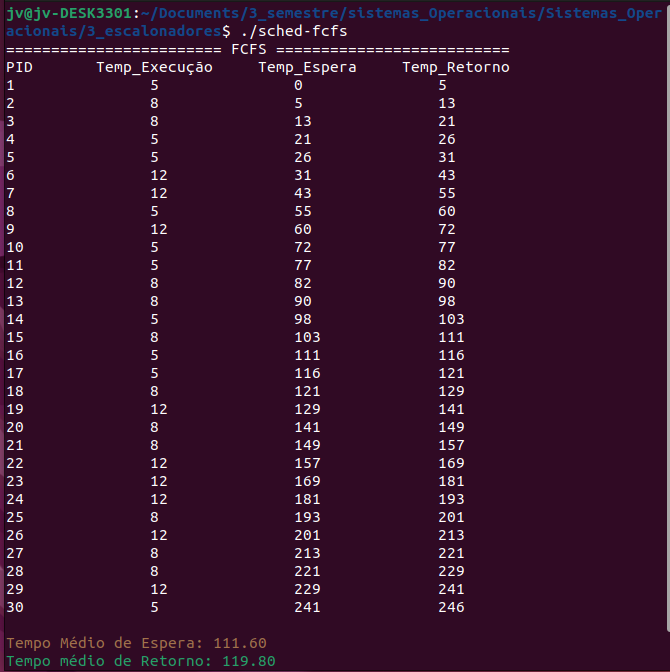
\includegraphics[width=0.7\textwidth]{imagens/fifo_run.png}
    \caption{Execução do Código em C.}
    \label{fig:fifo_run}
\end{figure}

\subsection{Explicação do código}

\begin{itemize}
    \item \textbf{Variáveis-chave:}
      \begin{itemize}
        \item `proc[]`: Um array que representa os identificadores dos processos (PID).
        \item `burst\_time[]`: Um array que armazena o tempo de execução de cada processo.
        \item `wait\_time[]`: Um array para armazenar o tempo de espera de cada processo.
        \item `tat[]`: Um array para armazenar o tempo de retorno (Turnaround\ Time) de cada processo.
        \item `total\_wt`: Variável para rastrear o tempo total de espera de todos os processos.
        \item `total\_tat`: Variável para rastrear o tempo total de retorno de todos os processos.
      \end{itemize}
  
    \item \textbf{Funções:}
      \begin{itemize}
        \item `waitingtime()`: Calcula o tempo de espera para cada processo, somando o tempo de execução do processo anterior com o tempo de espera do processo anterior.
        \item `turnaroundtime()`: Calcula o tempo de retorno para cada processo, que é a soma do tempo de execução e do tempo de espera.
        \item `avgtime()`: Função principal que implementa o algoritmo FIFO, calcula os tempos de espera e de retorno e exibe os resultados.
      \end{itemize}
  
    \item \textbf{Funcionamento:}
      \begin{itemize}
        \item Inicialmente, os processos são criados com tempos de execução variáveis, refletindo cenários realistas.
        \item Os processos são atendidos na ordem em que chegam à fila de prontidão, seguindo o princípio FIFO.
        \item O tempo de espera e o tempo de retorno são calculados para cada processo usando as funções `waitingtime()` e `turnaroundtime()`.
        \item Os resultados são impressos, mostrando o PID, o tempo de execução, o tempo de espera e o tempo de retorno de cada processo.
        \item Finalmente, são calculados os tempos médios de espera e de retorno e exibidos na saída.
      \end{itemize}
  \end{itemize}


\section{Comparação de Algoritmos}
Nesta seção, realizaremos uma análise comparativa do desempenho dos quatro algoritmos de escalonamento 
com base nos resultados dos Tempos Médios de Espera e Tempos Médios de Retorno obtidos na implementação 
mostradas anteriormente.

Na tabela abaixo vemos os tempos de cada algoritmo e na figura \ref{fig:graf} é apresentado um
gráfico que compara esses tempos.


\begin{table}[ht]
    \centering
    \begin{tabular}{|l|c|c|}
    \hline
    \textbf{Algoritmo} & \textbf{Tempo Médio de Espera} & \textbf{Tempo Médio de Retorno} \\
    \hline
    SJF (Shortest Job First) & 112.90 & 122.13 \\
    SRTF (Shortest Remaining Time First) & 101.60 & 110.13 \\
    Prioridades (Fixa) & 107.60 & 115.43 \\
    Round Robin & 213.63 & 223.03 \\
    FCFS (First Come First Served) & 111.60 & 119.80 \\
    \hline
    \end{tabular}
    \caption{Tempos Médios de Espera e Retorno para os Algoritmos de Escalonamento propostos.}
\end{table}

\begin{figure}[H]
        \centering
        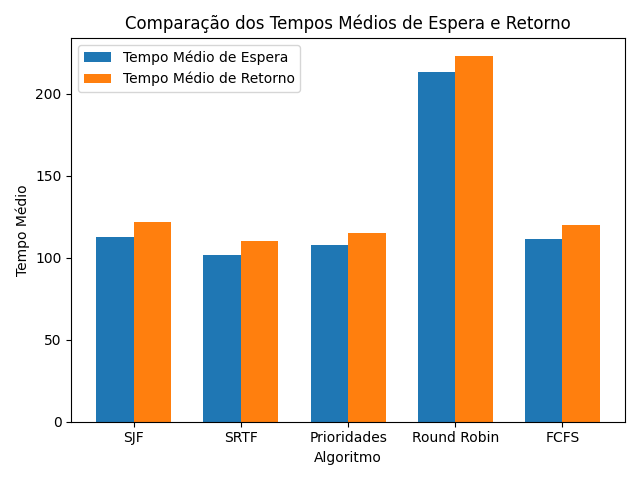
\includegraphics[width=0.7\textwidth]{imagens/grafico_bench.png}
        \caption{Comparação dos Tempos Médios de Espera e Retorno para os Algoritmos.}
        \label{fig:graf}
\end{figure}

Observando os resultados, podemos tirar algumas conclusões:

- O algoritmo SRTF (Shortest Remaining Time First) obteve os menores Tempos Médios de Espera e Retorno, o que indica um desempenho superior na minimização dos tempos de espera e retorno.

- O SJF (Shortest Job First) também demonstrou um bom desempenho, com tempos próximos aos do SRTF, mas um pouco mais longos devido à natureza não preemptiva do SJF.

- O algoritmo de Prioridades (Fixa) teve desempenho intermediário, com valores ligeiramente maiores de Tempos Médios de Espera e Retorno em comparação com o SRTF e o SJF.

- O FCFS (First Come, First Served) se manteve quase igual aos anteriores. No entanto, ele pode resultar em tempos de espera e retorno mais longos, especialmente quando processos longos são executados primeiro.

- O Round Robin apresentou os Tempos Médios de Espera e Retorno mais longos, o que é típico desse algoritmo, devido à divisão igualitária do tempo de CPU entre os processos.

\subsection{Escolha do Algoritmo}

A escolha do algoritmo de escalonamento depende dos requisitos específicos do sistema. Se o objetivo for minimizar os tempos de espera e 
etorno, o SRTF é a escolha preferencial. O SJF também é uma boa opção, mas pode não ser tão eficaz em sistemas não preemptivos. O algoritmo 
de Prioridades é útil quando a priorização de tarefas é necessária. O Round Robin é adequado para equilibrar a carga entre processos, mas com 
tempos de espera mais longos. O FCFS (First-Come, First-Served) é indicado quando a ordem de chegada dos processos é mais importante do que 
otimizar os tempos de espera e retorno, mas ele tende a resultar em tempos mais longos de espera e retorno.

Dessa forma, a seleção do algoritmo de escalonamento deve ser baseada nos objetivos do sistema, nas características dos processos e na natureza das cargas de trabalho.
    

\chapter{Conclusão}
\label{conclusao}

Neste relatório, exploramos a implementação e análise de cinco diferentes algoritmos de escalonamento de processos: SJF (Shortest Job First), SRTF (Shortest Remaining Time First), Prioridades (Fixa), Round Robin e FCFS (First-Come, First-Served). Cada um desses algoritmos tem suas próprias características e desempenho, e conduzimos uma análise comparativa com base nos resultados obtidos.

Observamos que o algoritmo SRTF (Shortest Remaining Time First) demonstrou o melhor desempenho em termos de minimização dos Tempos Médios de Espera e Retorno. Isso ocorre devido à natureza dinâmica do SRTF, que sempre prioriza os processos mais curtos, mas pode exigir trocas frequentes de contexto.

O SJF (Shortest Job First) também apresentou um bom desempenho, especialmente quando os tempos de execução dos processos são conhecidos com antecedência. No entanto, sua natureza não preemptiva pode não ser ideal em todos os cenários.

O algoritmo de Prioridades (Fixa) é valioso quando a priorização de tarefas é necessária, mas requer uma atribuição cuidadosa de prioridades para garantir um bom desempenho.

O Round Robin é útil para equilibrar a carga entre os processos, mas apresenta tempos de espera mais longos devido à divisão igualitária do tempo de CPU.

O FCFS (First-Come, First-Served) é indicado quando a ordem de chegada dos processos é mais importante do que otimizar os tempos de espera e retorno, mas ele tende a resultar em tempos mais longos de espera e retorno.

A escolha do algoritmo de escalonamento deve ser baseada nas necessidades específicas do sistema e nas características dos processos que serão executados. Cada algoritmo tem suas vantagens e desvantagens, e a seleção apropriada deve levar em consideração os objetivos de desempenho, as demandas do sistema e as configurações disponíveis.

Em última análise, a escalonamento de processos é uma parte essencial do gerenciamento de sistemas operacionais, e a compreensão das diferentes opções disponíveis é fundamental para a otimização do desempenho do sistema.

Este relatório fornece uma visão abrangente dos algoritmos de escalonamento e suas implicações, auxiliando na tomada de decisões informadas ao escolher o algoritmo mais adequado para um ambiente específico. A análise comparativa dos resultados destacou a importância de selecionar o algoritmo apropriado para atender aos objetivos do sistema e melhorar a experiência do usuário.

\postextual

\bibliography{bibliografia}

\cite{tanenbaum2010sistemas}

\end{document}
